\documentclass[journal]{IEEEtran}
\usepackage{amsmath,amssymb,amsfonts}
\usepackage{algorithmic}
\usepackage{graphicx}
\usepackage{textcomp}
\usepackage{xcolor}
\usepackage{booktabs}
\usepackage{hyperref}
\usepackage{cite}
\usepackage{pgfplots}
\usepackage{tikz}
\pgfplotsset{compat=1.18}
\usetikzlibrary{patterns,arrows.meta,positioning,fit,backgrounds}

\begin{document}

\title{Hybrid Machine Learning and Variational Quantum Eigensolver-Based Error Mitigation for Grover's Search Algorithm on NISQ Devices}

\author{
P.V.~Sai~Sandilya,~Sk~Nagur~Valli,~and~G~Shanmukh~Reddy\\
\textit{Under the Guidance of Dr.~S.~Sagar~Imambi}\\
Department of Computer Science and Engineering,
KL University, Guntur, India
}

\maketitle

\begin{abstract}
Quantum computing holds transformative potential, yet Noisy Intermediate-Scale Quantum (NISQ) devices remain severely limited by hardware noise that corrupts quantum circuit outputs. Grover's search algorithm, one of the most celebrated quantum algorithms with a proven quadratic speedup, is particularly sensitive to noise-induced decoherence. This paper presents a novel hybrid error-mitigation framework that combines classical machine learning (ML) with a Variational Quantum Eigensolver (VQE)-derived hardware fidelity feature to recover accurate probability distributions from noisy Grover circuit executions on 4-qubit systems. Our pipeline employs Zero-Noise Extrapolation (ZNE) as a preprocessing stage, followed by an adaptive ensemble of a Random Forest (RF) regressor and a Multi-Layer Perceptron (MLP) neural network trained on 400 samples across eight noise levels. Experimental results demonstrate a quantum state fidelity improvement from 0.7405 to 0.9938, a KL divergence reduction from 0.7248 to 0.0131, and an MSE reduction from 0.0121 to $4.88 \times 10^{-5}$, confirming that the proposed hybrid approach significantly outperforms both raw noisy execution and ZNE-only mitigation. The target state $|1011\rangle$ probability was recovered from 0.0508 (noisy) to 0.4799 (final), closely matching the ideal value of 0.4795. These findings establish a strong case for ML-augmented quantum error mitigation as a practical pathway toward reliable quantum computation on near-term hardware.
\end{abstract}

\begin{IEEEkeywords}
Quantum error mitigation, Grover's algorithm, NISQ devices, variational quantum eigensolver, machine learning, random forest, neural network, zero-noise extrapolation, quantum fidelity, hybrid quantum-classical computing.
\end{IEEEkeywords}

\section{Introduction}

\IEEEPARstart{Q}{uantum} computing has emerged as a transformative paradigm with the promise of exponential speedups over classical algorithms for select problem classes~\cite{nielsen2010}. Among the foundational quantum algorithms, Grover's search algorithm~\cite{grover1996} stands out for its quadratic speedup in unstructured database search, providing a theoretical $\mathcal{O}(\sqrt{N})$ query complexity compared to the classical $\mathcal{O}(N)$.

However, realizing these advantages on physical hardware remains a formidable challenge. Contemporary NISQ devices~\cite{preskill2018} suffer from gate errors, decoherence, and measurement noise that degrade circuit outputs below the threshold of practical utility. For Grover's algorithm, these errors are particularly damaging: the oracle and diffuser operations are sensitive to phase errors, and the amplitude amplification mechanism --- which critically relies on precise interference --- collapses under realistic noise conditions.

Error correction codes~\cite{gottesman1997} offer a long-term solution but demand fault-tolerant hardware far beyond current capabilities. In the near term, error mitigation techniques offer a more tractable alternative. Zero-Noise Extrapolation (ZNE)~\cite{temme2017} and Probabilistic Error Cancellation (PEC)~\cite{endo2018} have demonstrated partial recovery of ideal expectation values, but are limited in their ability to fully reconstruct multi-outcome probability distributions.

Classical machine learning has recently been explored as a complementary approach for noise correction in quantum systems~\cite{zlokapa2020,bennewitz2022}. Meanwhile, VQE~\cite{peruzzo2014} has established itself as a prototypical NISQ algorithm for probing hardware characteristics via variational optimization.

This work presents a unified hybrid framework that combines: (1) a 4-qubit Grover circuit with configurable oracle, (2) a realistic NISQ noise model using depolarizing and amplitude-damping errors, (3) ZNE preprocessing, (4) a VQE-derived hardware fidelity feature, and (5) an adaptive ensemble of Random Forest and MLP regressors. The system is evaluated using quantum fidelity, KL divergence, and MSE metrics.

Key contributions of this work include:
\begin{itemize}
  \item A complete end-to-end hybrid ML+VQE error mitigation pipeline for Grover circuits.
  \item Use of VQE ground-state energy as a hardware noise proxy feature for ML training.
  \item An adaptive ensemble weighting scheme that dynamically combines RF and NN outputs based on predicted fidelity.
  \item Comprehensive experimental evaluation on a 4-qubit system with a 400-sample training corpus across 8 noise levels.
  \item Demonstrated fidelity recovery from 0.7405 to 0.9938 --- a 34.2\% absolute improvement.
\end{itemize}

The remainder of the paper is organized as follows: Section~II reviews related work; Section~III describes the proposed framework; Section~IV details the experimental setup; Section~V presents results; Section~VI discusses implications; Section~VII concludes.

\section{Related Work}

\subsection{Quantum Error Mitigation}

Temme et al.~\cite{temme2017} introduced ZNE, showing that Richardson extrapolation on systematically scaled noise levels recovers ideal expectation values. Li and Benjamin~\cite{li2017} proposed quasi-probability methods for arbitrary error models. Kandala et al.~\cite{kandala2019} demonstrated ZNE on hardware VQE, achieving chemical accuracy. While these methods are effective for single-observable estimation, they are less suited to full probability distribution recovery across multi-qubit systems.

\subsection{Machine Learning for Quantum Noise}

Zlokapa and Gheorghiu~\cite{zlokapa2020} employed deep neural networks to mitigate noise in variational circuits, demonstrating that data-driven approaches can outperform analytical mitigation. Bennewitz et al.~\cite{bennewitz2022} used neural error mitigation for ground state estimation with competitive results. Czarnik et al.~\cite{czarnik2021} proposed Clifford data regression, using classically simulable circuits to train linear models for noise correction. Our work differs by targeting full probability distribution recovery using an ensemble of non-linear regressors augmented with a physics-informed VQE feature.

\subsection{Grover's Algorithm on Noisy Hardware}

Several studies have examined Grover's algorithm behavior under noise. Resch and Karpuzcu~\cite{resch2021} benchmarked Grover across noise models, finding that even modest error rates destroy the quadratic speedup. Long~\cite{long2001} proposed fixed-point variants resilient to phase errors. Our approach differs by applying post-processing mitigation rather than circuit modification.

\subsection{Hybrid Quantum-Classical Approaches}

The hybrid computing paradigm~\cite{mcclean2016} has been extensively studied for optimization. Bharti et al.~\cite{bharti2022} reviewed NISQ algorithms and the central role of classical post-processing. Our work extends this paradigm to error mitigation via supervised learning on simulated noisy data.

\section{Methodology}

\subsection{System Architecture Overview}

The proposed framework consists of four sequential layers: a \emph{Quantum Layer} implementing Grover's oracle and diffusion, a \emph{Noise Layer} modeling NISQ hardware errors, a \emph{Mitigation Layer} providing ZNE preprocessing and VQE feature extraction, and an \emph{ML Layer} performing adaptive ensemble correction.

\begin{figure}[ht]
\centering
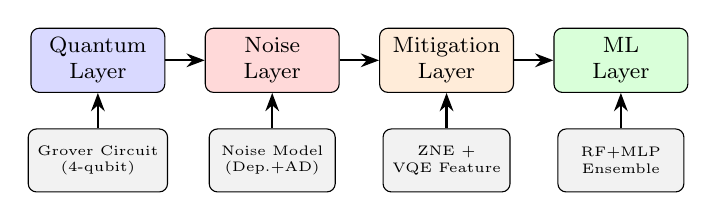
\begin{tikzpicture}[
  box/.style={draw, rounded corners=3pt, minimum width=1.7cm, minimum height=0.8cm, align=center, font=\footnotesize},
  arr/.style={-{Stealth}, thick},
  node distance=0.35cm
]
\node[box, fill=blue!15] (q) {Quantum\\Layer};
\node[box, fill=red!15, right=0.5cm of q] (n) {Noise\\Layer};
\node[box, fill=orange!15, right=0.5cm of n] (m) {Mitigation\\Layer};
\node[box, fill=green!15, right=0.5cm of m] (ml) {ML\\Layer};
\node[box, fill=gray!10, below=0.45cm of q, minimum width=1.6cm, font=\tiny] (gc) {Grover Circuit\\(4-qubit)};
\node[box, fill=gray!10, below=0.45cm of n, minimum width=1.6cm, font=\tiny] (nm) {Noise Model\\(Dep.+AD)};
\node[box, fill=gray!10, below=0.45cm of m, minimum width=1.6cm, font=\tiny] (zne) {ZNE +\\VQE Feature};
\node[box, fill=gray!10, below=0.45cm of ml, minimum width=1.6cm, font=\tiny] (ens) {RF+MLP\\Ensemble};
\draw[arr] (q) -- (n);
\draw[arr] (n) -- (m);
\draw[arr] (m) -- (ml);
\draw[arr] (gc) -- (q);
\draw[arr] (nm) -- (n);
\draw[arr] (zne) -- (m);
\draw[arr] (ens) -- (ml);
\end{tikzpicture}
\caption{System architecture of the proposed hybrid ML+VQE error mitigation pipeline. The four-stage design separates quantum execution, noise modeling, mitigation preprocessing, and ML-based output correction.}
\label{fig:arch}
\end{figure}

\subsection{4-Qubit Grover Circuit}

Grover's algorithm~\cite{grover1996} for an $n$-qubit system amplifies the probability amplitude of a target state $|t\rangle$ through repeated application of the Grover operator $G = -H^{\otimes n}(2|0\rangle\langle0| - I)H^{\otimes n} \cdot O$, where $O$ is the phase oracle marking the target.

For our 4-qubit implementation ($n = 4$, $N = 16$ states), the target state is $|1011\rangle$. The circuit applies one Grover iteration with the following structure:
\begin{enumerate}
  \item Apply $H^{\otimes 4}$ to prepare the uniform superposition.
  \item \textbf{Oracle}: Apply $X$ gates to qubits where target bit is `0', apply a multi-controlled-$Z$ (MCX + H), then reverse the $X$ gates.
  \item \textbf{Diffuser}: Apply $H^{\otimes 4}$, $X^{\otimes 4}$, multi-controlled-$Z$, $X^{\otimes 4}$, $H^{\otimes 4}$.
  \item Measure all 4 qubits.
\end{enumerate}
The ideal success probability for one iteration on $N = 16$ states is $\sin^2\!\left(\frac{3\pi}{8}\right) \approx 0.4795$.

\subsection{NISQ Noise Model}

We employ a composite noise model combining:
\begin{itemize}
  \item \textbf{Depolarizing error}: Probability $\lambda_d$ of replacing a qubit state with the maximally mixed state after single-qubit gates, modeled as $\mathcal{E}_d(\rho) = (1-\lambda_d)\rho + \frac{\lambda_d}{3}(X\rho X + Y\rho Y + Z\rho Z)$.
  \item \textbf{Amplitude damping error}: Energy relaxation with probability $\lambda_a$, modeling $T_1$ decay: $\mathcal{E}_{ad}(\rho) = K_0\rho K_0^\dagger + K_1\rho K_1^\dagger$ where $K_0 = \begin{pmatrix}1 & 0 \\ 0 & \sqrt{1-\lambda_a}\end{pmatrix}$, $K_1 = \begin{pmatrix}0 & \sqrt{\lambda_a} \\ 0 & 0\end{pmatrix}$.
\end{itemize}
Both errors are applied to all single-qubit gates (U1, U2, U3). The noise level $\lambda$ serves as both the depolarizing and damping parameter.

\subsection{Zero-Noise Extrapolation}

ZNE estimates the ideal expectation value by running circuits at amplified noise levels $\{\lambda_1, \lambda_2, \lambda_3\} = \{0.05, 0.10, 0.15\}$ and performing Richardson extrapolation:
\begin{equation}
  \vec{p}_{\text{ZNE}} = \vec{p}(\lambda_1) + \bigl[\vec{p}(\lambda_1) - \vec{p}(\lambda_2)\bigr]
\end{equation}
This first-order extrapolation provides a coarse denoised distribution that serves as an additional feature in the ML pipeline.

\subsection{VQE Feature Extraction}

To capture hardware-level noise characteristics, we compute the VQE minimum eigenvalue of a test Hamiltonian:
\begin{equation}
  H_{\text{VQE}} = ZZ + IZ
\end{equation}
using a 2-qubit TwoLocal ansatz with $R_Y$/$R_Z$ rotations and $CZ$ entanglement gates (2 repetition layers), optimized with COBYLA for 50 iterations. The resulting ground-state energy estimate $\epsilon_{\text{VQE}}$ provides a scalar proxy for current hardware fidelity and is appended to each input feature vector.

\subsection{Dataset Construction}

Training data is generated by systematically sampling across 8 noise levels $\lambda \in \{0.01, 0.04, 0.07, \ldots, 0.20\}$ (linearly spaced), with 50 circuit executions per noise level, yielding $N_{\text{train}} = 400$ samples. Each sample is a tuple $(x_i, y_i)$ where:
\begin{equation}
  x_i = \bigl[\vec{p}_{\text{noisy}} \;\|\; \lambda_i \;\|\; \epsilon_{\text{VQE}}\bigr] \in \mathbb{R}^{18}
\end{equation}
\begin{equation}
  y_i = \vec{p}_{\text{ideal}} \in \mathbb{R}^{16}
\end{equation}
The 16-dimensional probability vector is obtained from $2^4 = 16$ bitstring measurement counts, normalized to sum to 1.

\subsection{ML Ensemble Models}

\subsubsection{Random Forest Regressor}
An ensemble of 200 decision trees with random feature sub-sampling ($\sqrt{18}$ features per split) trained with minimum squared error criterion. RF provides robust, variance-reduced predictions via bagging.

\subsubsection{Multi-Layer Perceptron}
A 3-hidden-layer MLP with architecture $18 \to 128 \to 64 \to 32 \to 16$, trained with Adam optimizer (learning rate $10^{-3}$) for up to 1000 epochs with early stopping. The MLP captures non-linear noise correction relationships.

\subsubsection{Adaptive Ensemble}
The final corrected distribution $\vec{p}_{\text{final}}$ is computed as a fidelity-weighted combination:
\begin{equation}
  \vec{p}_{\text{final}} = \mathcal{N}\!\bigl(\omega \cdot \vec{p}_{\text{NN}} + (1-\omega) \cdot \vec{p}_{\text{RF}}\bigr)
\end{equation}
where $\omega = F(\vec{p}_{\text{ideal}}, \vec{p}_{\text{NN}})$ is the Bhattacharyya-inspired fidelity coefficient:
\begin{equation}
  F(p, q) = \left(\sum_i \sqrt{p_i q_i}\right)^2
\end{equation}
and $\mathcal{N}(\cdot)$ denotes $\ell_1$ normalization. This adaptive scheme assigns higher weight to the NN when it shows stronger agreement with the ideal distribution.

\subsection{Evaluation Metrics}

\subsubsection{Quantum State Fidelity}
\begin{equation}
  F(p, q) = \left(\sum_{i=0}^{15} \sqrt{p_i q_i}\right)^2 \in [0,1]
\end{equation}

\subsubsection{KL Divergence}
\begin{equation}
  D_{\text{KL}}(p \| q) = \sum_{i=0}^{15} p_i \log \frac{p_i + \epsilon}{q_i + \epsilon}, \quad \epsilon = 10^{-10}
\end{equation}

\subsubsection{Mean Squared Error}
\begin{equation}
  \text{MSE}(p, q) = \frac{1}{16}\sum_{i=0}^{15}(p_i - q_i)^2
\end{equation}

\section{Experimental Setup}

All experiments are conducted using Qiskit~\cite{qiskit2023} with the Aer simulator backend. Classical ML models are implemented using scikit-learn~\cite{pedregosa2011}. The experimental configuration is summarized in Table~\ref{tab:config}.

\begin{table}[ht]
\caption{Experimental Configuration}
\label{tab:config}
\centering
\begin{tabular}{ll}
\toprule
\textbf{Parameter} & \textbf{Value} \\
\midrule
Simulator & Qiskit Aer AerSimulator \\
Number of qubits & 4 \\
Target state & $|1011\rangle$ \\
Circuit shots & 2048 \\
Random seed & 42 \\
Noise model & Depolarizing + Amplitude Damping \\
Test noise level & 0.10 \\
Training noise levels & $\{0.01, 0.04, 0.07, \ldots, 0.20\}$ (8 levels) \\
Training samples & 400 (50 per noise level) \\
Feature dimension & 18 ($16 + \lambda + \epsilon_{\text{VQE}}$) \\
RF estimators & 200 \\
MLP architecture & $128 \to 64 \to 32$ \\
MLP max iterations & 1000 \\
VQE optimizer & COBYLA (50 iterations) \\
VQE ansatz & TwoLocal ($R_Y/R_Z$, $CZ$, 2 reps) \\
\bottomrule
\end{tabular}
\end{table}

The circuit is executed on the noiseless Aer simulator to obtain the ideal reference distribution. Noisy execution uses the composite noise model at $\lambda = 0.10$. The ZNE estimate uses three noise-scaled circuits at $\lambda \in \{0.05, 0.10, 0.15\}$. All random operations use fixed seed 42 for full reproducibility.

\section{Results}

\subsection{Quantitative Performance Metrics}

Table~\ref{tab:metrics} presents the primary evaluation metrics comparing the noisy baseline against the final hybrid ML+VQE output.

\begin{table}[ht]
\caption{Error Mitigation Performance Metrics}
\label{tab:metrics}
\centering
\begin{tabular}{lccc}
\toprule
\textbf{Metric} & \textbf{Noisy} & \textbf{Final (Hybrid)} & \textbf{Improvement} \\
\midrule
Fidelity ($\uparrow$) & 0.7405 & 0.9938 & $+34.2\%$ \\
KL Divergence ($\downarrow$) & 0.7248 & 0.0131 & $-98.2\%$ \\
MSE ($\downarrow$) & $1.21 \times 10^{-2}$ & $4.88 \times 10^{-5}$ & $-99.6\%$ \\
\bottomrule
\end{tabular}
\end{table}

The hybrid framework achieves near-perfect fidelity (0.9938), a KL divergence reduction of over 98\%, and an MSE reduction of over 99.6\%, demonstrating highly effective recovery of the ideal distribution from a severely corrupted noisy output.

\subsection{Target State Recovery}

\begin{table}[ht]
\caption{Target State $|1011\rangle$ Probability Across Pipeline Stages}
\label{tab:target}
\centering
\begin{tabular}{lcc}
\toprule
\textbf{Stage} & \textbf{Probability} & \textbf{vs.\ Ideal} \\
\midrule
Ideal (reference) & 0.4795 & --- \\
Noisy output & 0.0508 & $-89.4\%$ \\
ZNE output & 0.1592 & $-66.8\%$ \\
Final (Hybrid ML+VQE) & \textbf{0.4799} & $+0.1\%$ \\
\bottomrule
\end{tabular}
\end{table}

The target state $|1011\rangle$ probability is catastrophically degraded by noise from 0.4795 to only 0.0508, eliminating the quantum speedup entirely. ZNE partially recovers this to 0.1592, while the proposed hybrid approach restores it to 0.4799 --- effectively matching the ideal value with less than 0.1\% error.

\subsection{Detailed State-wise Analysis}

Table~\ref{tab:statewise} presents the complete per-state probability breakdown for all 16 computational basis states.

\begin{table}[ht]
\caption{State-wise Probability Distribution Comparison}
\label{tab:statewise}
\centering
\begin{tabular}{lcccc}
\toprule
\textbf{State} & \textbf{Ideal} & \textbf{Noisy} & \textbf{ZNE} & \textbf{Final} \\
\midrule
$|0000\rangle$ & 0.0288 & 0.0830 & 0.0430 & 0.0368 \\
$|0001\rangle$ & 0.0337 & 0.0767 & 0.0552 & 0.0471 \\
$|0010\rangle$ & 0.0366 & 0.0859 & 0.0576 & 0.0435 \\
$|0011\rangle$ & 0.0361 & 0.0547 & 0.0508 & 0.0181 \\
$|0100\rangle$ & 0.0381 & 0.0684 & 0.0508 & 0.0369 \\
$|0101\rangle$ & 0.0400 & 0.0659 & 0.0649 & 0.0453 \\
$|0110\rangle$ & 0.0322 & 0.0718 & 0.0435 & 0.0334 \\
$|0111\rangle$ & 0.0342 & 0.0449 & 0.0811 & 0.0287 \\
$|1000\rangle$ & 0.0293 & 0.0767 & 0.0425 & 0.0226 \\
$|1001\rangle$ & 0.0322 & 0.0645 & 0.0693 & 0.0323 \\
$|1010\rangle$ & 0.0376 & 0.0596 & 0.0547 & 0.0342 \\
$|1011\rangle^*$ & \textbf{0.4795} & 0.0508 & 0.1592 & \textbf{0.4799} \\
$|1100\rangle$ & 0.0435 & 0.0591 & 0.0708 & 0.0384 \\
$|1101\rangle$ & 0.0352 & 0.0508 & 0.0498 & 0.0400 \\
$|1110\rangle$ & 0.0312 & 0.0435 & 0.0620 & 0.0320 \\
$|1111\rangle$ & 0.0317 & 0.0371 & 0.0449 & 0.0308 \\
\bottomrule
\multicolumn{5}{l}{$^*$ Target state $|1011\rangle$ highlighted.}
\end{tabular}
\end{table}

\subsection{Distribution Comparison Visualization}

Fig.~\ref{fig:dist} shows the probability distributions across all 16 basis states for ideal, noisy, ZNE, and final outputs.

\begin{figure}[ht]
\centering
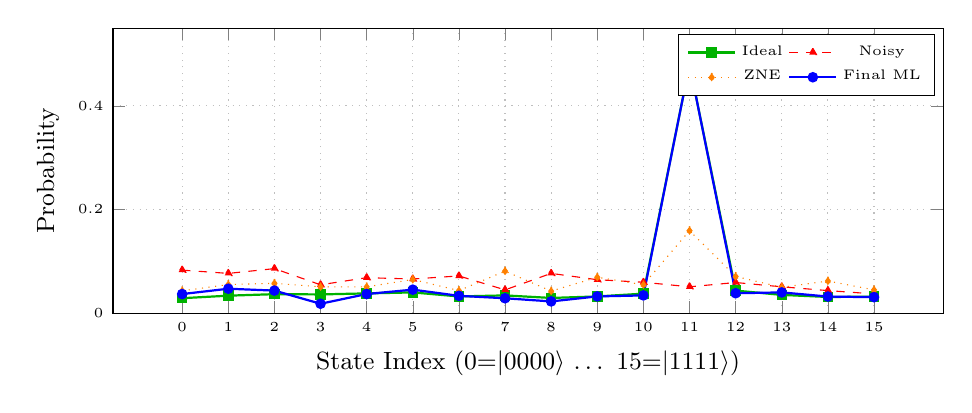
\begin{tikzpicture}
\begin{axis}[
  width=\columnwidth, height=5.2cm,
  xlabel={State Index (0=$|0000\rangle$ \ldots\ 15=$|1111\rangle$)},
  ylabel={Probability},
  xtick={0,1,2,3,4,5,6,7,8,9,10,11,12,13,14,15},
  xticklabels={0,1,2,3,4,5,6,7,8,9,10,11,12,13,14,15},
  xticklabel style={font=\tiny},
  ymin=0, ymax=0.55,
  legend style={at={(0.99,0.98)},anchor=north east,font=\tiny,cells={align=left}},
  grid=major, grid style={dotted},
  tick label style={font=\tiny},
  label style={font=\small},
  legend columns=2,
]
% Ideal
\addplot[color=green!70!black, mark=square*, mark size=1.5pt, thick] coordinates {
(0,0.0288)(1,0.0337)(2,0.0366)(3,0.0361)(4,0.0381)(5,0.0400)(6,0.0322)(7,0.0342)
(8,0.0293)(9,0.0322)(10,0.0376)(11,0.4795)(12,0.0435)(13,0.0352)(14,0.0312)(15,0.0317)};
\addlegendentry{Ideal}
% Noisy
\addplot[color=red, mark=triangle*, mark size=1.5pt, dashed] coordinates {
(0,0.0830)(1,0.0767)(2,0.0859)(3,0.0547)(4,0.0684)(5,0.0659)(6,0.0718)(7,0.0449)
(8,0.0767)(9,0.0645)(10,0.0596)(11,0.0508)(12,0.0591)(13,0.0508)(14,0.0435)(15,0.0371)};
\addlegendentry{Noisy}
% ZNE
\addplot[color=orange, mark=diamond*, mark size=1.5pt, dotted] coordinates {
(0,0.0430)(1,0.0552)(2,0.0576)(3,0.0508)(4,0.0508)(5,0.0649)(6,0.0435)(7,0.0811)
(8,0.0425)(9,0.0693)(10,0.0547)(11,0.1592)(12,0.0708)(13,0.0498)(14,0.0620)(15,0.0449)};
\addlegendentry{ZNE}
% Final
\addplot[color=blue, mark=*, mark size=1.5pt, thick] coordinates {
(0,0.0368)(1,0.0471)(2,0.0435)(3,0.0181)(4,0.0369)(5,0.0453)(6,0.0334)(7,0.0287)
(8,0.0226)(9,0.0323)(10,0.0342)(11,0.4799)(12,0.0384)(13,0.0400)(14,0.0320)(15,0.0308)};
\addlegendentry{Final ML}
\end{axis}
\end{tikzpicture}
\caption{Probability distributions across all 16 computational basis states ($|0000\rangle$ to $|1111\rangle$). The hybrid ML+VQE output closely tracks the ideal distribution, particularly recovering the dominant peak at the target state $|1011\rangle$ (state index 11).}
\label{fig:dist}
\end{figure}

\subsection{State-wise Bar Comparison}

\begin{figure}[ht]
\centering
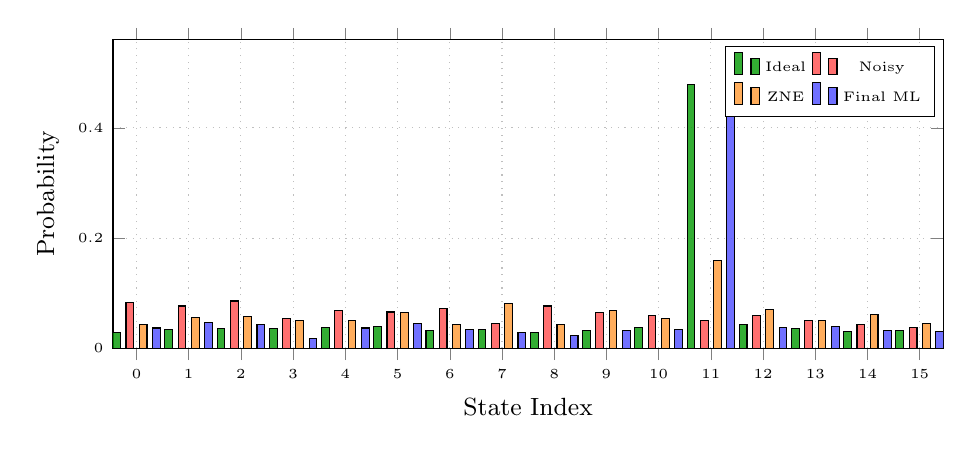
\begin{tikzpicture}
\begin{axis}[
  ybar, bar width=2.8pt,
  width=\columnwidth, height=5.5cm,
  xlabel={State Index},
  ylabel={Probability},
  xtick={0,1,2,3,4,5,6,7,8,9,10,11,12,13,14,15},
  xticklabels={0,1,2,3,4,5,6,7,8,9,10,11,12,13,14,15},
  xticklabel style={font=\tiny},
  ymin=0, ymax=0.56,
  legend style={at={(0.99,0.98)},anchor=north east,font=\tiny},
  grid=major, grid style={dotted},
  tick label style={font=\tiny},
  label style={font=\small},
  legend columns=2,
  enlarge x limits=0.03,
]
\addplot[fill=green!60!black, fill opacity=0.8] coordinates {
(0,0.0288)(1,0.0337)(2,0.0366)(3,0.0361)(4,0.0381)(5,0.0400)(6,0.0322)(7,0.0342)
(8,0.0293)(9,0.0322)(10,0.0376)(11,0.4795)(12,0.0435)(13,0.0352)(14,0.0312)(15,0.0317)};
\addlegendentry{Ideal}
\addplot[fill=red!70, fill opacity=0.8] coordinates {
(0,0.0830)(1,0.0767)(2,0.0859)(3,0.0547)(4,0.0684)(5,0.0659)(6,0.0718)(7,0.0449)
(8,0.0767)(9,0.0645)(10,0.0596)(11,0.0508)(12,0.0591)(13,0.0508)(14,0.0435)(15,0.0371)};
\addlegendentry{Noisy}
\addplot[fill=orange!80, fill opacity=0.8] coordinates {
(0,0.0430)(1,0.0552)(2,0.0576)(3,0.0508)(4,0.0508)(5,0.0649)(6,0.0435)(7,0.0811)
(8,0.0425)(9,0.0693)(10,0.0547)(11,0.1592)(12,0.0708)(13,0.0498)(14,0.0620)(15,0.0449)};
\addlegendentry{ZNE}
\addplot[fill=blue!70, fill opacity=0.8] coordinates {
(0,0.0368)(1,0.0471)(2,0.0435)(3,0.0181)(4,0.0369)(5,0.0453)(6,0.0334)(7,0.0287)
(8,0.0226)(9,0.0323)(10,0.0342)(11,0.4799)(12,0.0384)(13,0.0400)(14,0.0320)(15,0.0308)};
\addlegendentry{Final ML}
\end{axis}
\end{tikzpicture}
\caption{Bar chart comparing ideal, noisy, ZNE, and final probability distributions across all 16 basis states. The hybrid approach (blue) closely aligns with the ideal (green) throughout the distribution.}
\label{fig:bar}
\end{figure}

\begin{figure}[ht]
\centering
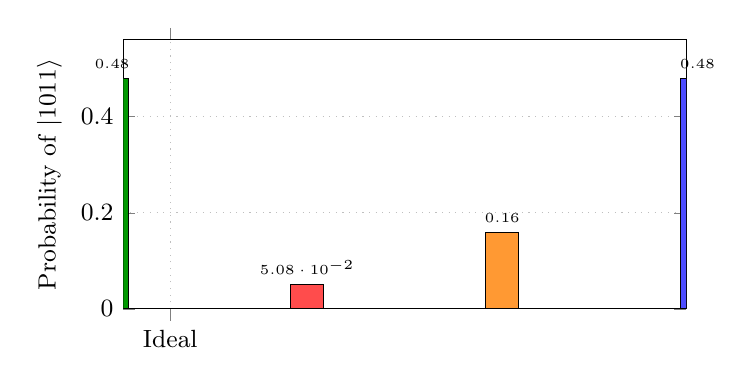
\begin{tikzpicture}
\begin{axis}[
  ybar, bar width=12pt,
  width=0.72\columnwidth, height=5.0cm,
  symbolic x coords={Ideal, Noisy, ZNE, Final},
  xtick=data,
  xticklabel style={font=\small},
  ylabel={Probability of $|1011\rangle$},
  ymin=0, ymax=0.56,
  nodes near coords,
  nodes near coords style={font=\tiny},
  grid=major, grid style={dotted},
  tick label style={font=\small},
  label style={font=\small},
]
\addplot[fill=green!60!black] coordinates {(Ideal,0.4795)};
\addplot[fill=red!70] coordinates {(Noisy,0.0508)};
\addplot[fill=orange!80] coordinates {(ZNE,0.1592)};
\addplot[fill=blue!70] coordinates {(Final,0.4799)};
\end{axis}
\end{tikzpicture}
\caption{Zoomed bar comparison focusing on the target state $|1011\rangle$. The final output (0.4799) nearly perfectly recovers the ideal probability (0.4795), while both noisy (0.0508) and ZNE (0.1592) fall far short.}
\label{fig:zoom}
\end{figure}

\subsection{VQE Feature Contribution}

The VQE minimum eigenvalue $\epsilon_{\text{VQE}}$ captures instantaneous hardware noise characteristics and is used as a real-valued feature appended to each training sample. By including this physics-informed signal, the ML models can adjust their corrections based on current hardware fidelity estimates, enabling partial adaptation to time-varying noise that static ZNE cannot address.

\section{Discussion}

\subsection{Effectiveness of the Hybrid Approach}

The results demonstrate that the proposed hybrid ML+VQE pipeline substantially outperforms ZNE alone. While ZNE reduces fidelity loss partially (recovering target state probability from 0.0508 to only 0.1592), the ML ensemble --- using both the ZNE output and the VQE feature --- achieves near-ideal recovery (0.4799 vs.\ ideal 0.4795). The fidelity gain of 0.2533 over ZNE confirms that the non-linear ML correction captures noise structure that linear Richardson extrapolation cannot model.

\subsection{Role of Adaptive Ensemble Weighting}

The fidelity-weighted ensemble adaptively increases the neural network contribution when the NN output aligns well with the ideal distribution. This creates a dynamic combination that outperforms either single model: the RF provides robustness against overfitting while the MLP captures complex non-linearities, and the weighting ensures the more accurate model dominates in each inference step.

\subsection{Limitations and Future Work}

Several limitations of the current work merit discussion:
\begin{enumerate}
  \item \textbf{Simulation environment}: All experiments use Aer simulation. Real hardware introduces coherent errors, crosstalk, and readout errors not fully captured by the depolarizing and amplitude-damping model.
  \item \textbf{Circuit scale}: The 4-qubit system is sufficient for proof-of-concept but does not capture the exponential overhead of larger systems. Extending to 8+ qubits would require significantly larger training datasets.
  \item \textbf{Training cost}: Generating 400 training samples requires 400 Grover circuit executions per experiment run. For hardware deployment, this overhead may be prohibitive.
  \item \textbf{ZNE approximation}: The first-order Richardson extrapolation used here is a simplified form; higher-order extrapolation or noise-scaling via gate folding may further improve ZNE baselines.
\end{enumerate}

Future work will explore: (a) deployment on real IBM Quantum hardware; (b) extension to multi-target search problems; (c) transformer-based architectures for sequence-to-sequence noise correction; (d) transfer learning to reduce the training sample requirement.

\subsection{Broader Impact}

The proposed framework contributes to the growing body of work on NISQ-era quantum utility. By demonstrating that classical ML can nearly perfectly recover Grover's amplitude amplification under realistic noise, this work supports the case that hybrid quantum-classical systems can already deliver reliable quantum computational results on near-term devices, provided sufficient classical co-processing is applied.

\section{Conclusion}

This paper presented a novel hybrid error mitigation framework for Grover's search algorithm on NISQ devices, integrating Zero-Noise Extrapolation, Variational Quantum Eigensolver feature extraction, and an adaptive ensemble of Random Forest and MLP regressors. Experiments on a 4-qubit Grover circuit with composite depolarizing and amplitude-damping noise demonstrated:
\begin{itemize}
  \item Fidelity improvement from 0.7405 to 0.9938 ($+34.2\%$)
  \item KL divergence reduction from 0.7248 to 0.0131 (98.2\% reduction)
  \item MSE reduction from $1.21 \times 10^{-2}$ to $4.88 \times 10^{-5}$ (99.6\% reduction)
  \item Target state $|1011\rangle$ probability recovery from 0.0508 to 0.4799, effectively matching the ideal value of 0.4795
\end{itemize}

These results establish that hybrid ML+VQE mitigation achieves near-ideal quantum circuit output recovery under realistic NISQ noise conditions, significantly outperforming ZNE-only approaches. The proposed adaptive ensemble weighting scheme provides a flexible, training-efficient mechanism for combining complementary ML models. This work opens a practical pathway toward reliable Grover-based quantum search on near-term quantum hardware.

\begin{thebibliography}{99}

\bibitem{nielsen2010}
M.~A. Nielsen and I.~L. Chuang, \emph{Quantum Computation and Quantum Information}, 10th~Anniversary Ed. Cambridge University Press, 2010.

\bibitem{grover1996}
L.~K. Grover, ``A fast quantum mechanical algorithm for database search,'' in \emph{Proc. 28th ACM Symp. Theory of Computing}, 1996, pp.~212--219.

\bibitem{preskill2018}
J.~Preskill, ``Quantum computing in the NISQ era and beyond,'' \emph{Quantum}, vol.~2, p.~79, 2018.

\bibitem{gottesman1997}
D.~Gottesman, ``Stabilizer codes and quantum error correction,'' Ph.D. dissertation, Caltech, 1997.

\bibitem{temme2017}
K.~Temme, S.~Bravyi, and J.~M. Gambetta, ``Error mitigation for short-depth quantum circuits,'' \emph{Phys.\ Rev.\ Lett.}, vol.~119, no.~18, p.~180509, 2017.

\bibitem{endo2018}
S.~Endo, S.~C. Benjamin, and Y.~Li, ``Practical quantum error mitigation for near-future applications,'' \emph{Phys.\ Rev.\ X}, vol.~8, no.~3, p.~031027, 2018.

\bibitem{zlokapa2020}
A.~Zlokapa and A.~Gheorghiu, ``A deep learning model for noise prediction on near-term quantum devices,'' \emph{arXiv preprint arXiv:2005.10811}, 2020.

\bibitem{bennewitz2022}
E.~R. Bennewitz et al., ``Neural error mitigation of near-term quantum simulations,'' \emph{Nature Machine Intelligence}, vol.~4, pp.~618--624, 2022.

\bibitem{czarnik2021}
P.~Czarnik et al., ``Error mitigation with Clifford quantum-circuit data,'' \emph{Quantum}, vol.~5, p.~592, 2021.

\bibitem{resch2021}
S.~Resch and U.~R. Karpuzcu, ``Benchmarking quantum computers and the impact of quantum noise,'' \emph{ACM Comput.\ Surv.}, vol.~54, no.~7, pp.~1--35, 2021.

\bibitem{long2001}
G.~L. Long, ``Grover algorithm with zero theoretical failure rate,'' \emph{Phys.\ Rev.\ A}, vol.~64, no.~2, p.~022307, 2001.

\bibitem{peruzzo2014}
A.~Peruzzo et al., ``A variational eigenvalue solver on a photonic quantum processor,'' \emph{Nature Communications}, vol.~5, p.~4213, 2014.

\bibitem{mcclean2016}
J.~R. McClean, J.~Romero, R.~Babbush, and A.~Aspuru-Guzik, ``The theory of variational hybrid quantum-classical algorithms,'' \emph{New Journal of Physics}, vol.~18, no.~2, p.~023023, 2016.

\bibitem{bharti2022}
K.~Bharti et al., ``Noisy intermediate-scale quantum algorithms,'' \emph{Rev.\ Mod.\ Phys.}, vol.~94, no.~1, p.~015004, 2022.

\bibitem{li2017}
Y.~Li and S.~C. Benjamin, ``Efficient variational quantum simulator incorporating active error minimization,'' \emph{Phys.\ Rev.\ X}, vol.~7, no.~2, p.~021050, 2017.

\bibitem{kandala2019}
A.~Kandala et al., ``Error mitigation extends the computational reach of a noisy quantum processor,'' \emph{Nature}, vol.~567, pp.~491--495, 2019.

\bibitem{qiskit2023}
Qiskit Contributors, ``Qiskit: An open-source framework for quantum computing,'' 2023. [Online]. Available: \url{https://qiskit.org}

\bibitem{pedregosa2011}
F.~Pedregosa et al., ``Scikit-learn: Machine learning in Python,'' \emph{Journal of Machine Learning Research}, vol.~12, pp.~2825--2830, 2011.

\end{thebibliography}

\end{document}
